\documentclass{article}

% This is the workshop style (ICBINB for ICLR 2025) - do not change.
% We keep single-column format and up to 4 pages for the main text (not counting references).
% We minimally edit the content to optimize page usage while preserving key discussions.

\usepackage[margin=1in]{geometry}
\usepackage{graphicx}
\usepackage{subcaption}
\usepackage{amsmath,amssymb}
\usepackage{booktabs}
\usepackage{url}
\usepackage{microtype}

\graphicspath{{figures/}}

\title{A Hybrid Model's Real-World Challenges:
Overfitting and Inconclusive Gains}

\author{
  An Ambitious AI Researcher \\
  Department of Ambition, AI University \\
  \texttt{researcher@aiuniversity.edu}
}

\date{}

\begin{document}

\maketitle

\begin{abstract}
In this work, we explore the challenges and pitfalls of a hybrid deep learning model for text classification tasks. Despite promising theoretical motivations, our empirical results reveal overfitting tendencies and inconclusive gains in real-world scenarios. These insights emphasize the difficulty of robust deployment and underscore the importance of transparent reporting of negative and ambivalent findings.
\end{abstract}

\section{Introduction}
Recent advances in deep learning have yielded strong results on benchmark datasets. However, these improvements often fail to translate into consistent real-world gains~\cite{brown2020language,vaswani2017attention}. In this paper, we examine a hybrid model that combines pre-trained embeddings with specialized modules. The idea was to leverage a flexible architecture to address domain shift and class imbalance. Yet our experiments reveal unremarkable or inconsistent gains in practical contexts. We present lessons learned and emphasize that partial failures or negative results can offer the community meaningful insight for future efforts.

\section{Related Work}
Numerous works highlight the gap between benchmark performance and real-world transferability~\cite{devlin2019bert, he2016deep}. Studies that examine negative or inconclusive results remain fewer, although they are increasingly recognized for strengthening scientific rigor~\cite{henderson2018deep}. Our approach draws from attempts to combine pretrained language models with domain-specific modules (e.g.,~\cite{peters2018deep}) but demonstrates that such hybrid solutions can lead to modest or even negligible gains in practice.

\section{Method}
We design a hybrid architecture by integrating a pretrained text encoder with a lightweight domain classifier, optimized under an end-to-end paradigm. Training is performed on domain-specific text data, augmented with label smoothing to mitigate class imbalance. Hyperparameters and further architectural details appear in the Appendix.

\section{Experiments}
We evaluate on a proprietary text classification dataset, measuring macro-F1 score, loss curves, and confusion matrices. Although early epochs suggested promising gains, performance stabilized well before surpassing a strong baseline. These observations highlight potential overfitting and model sensitivity to initialization.

\begin{figure}[t]
\centering
\begin{subfigure}[b]{0.48\textwidth}
    \includegraphics[width=\textwidth]{baseline_performance.png}
    \caption{Baseline training/validation metrics.}
\end{subfigure}
\hfill
\begin{subfigure}[b]{0.48\textwidth}
    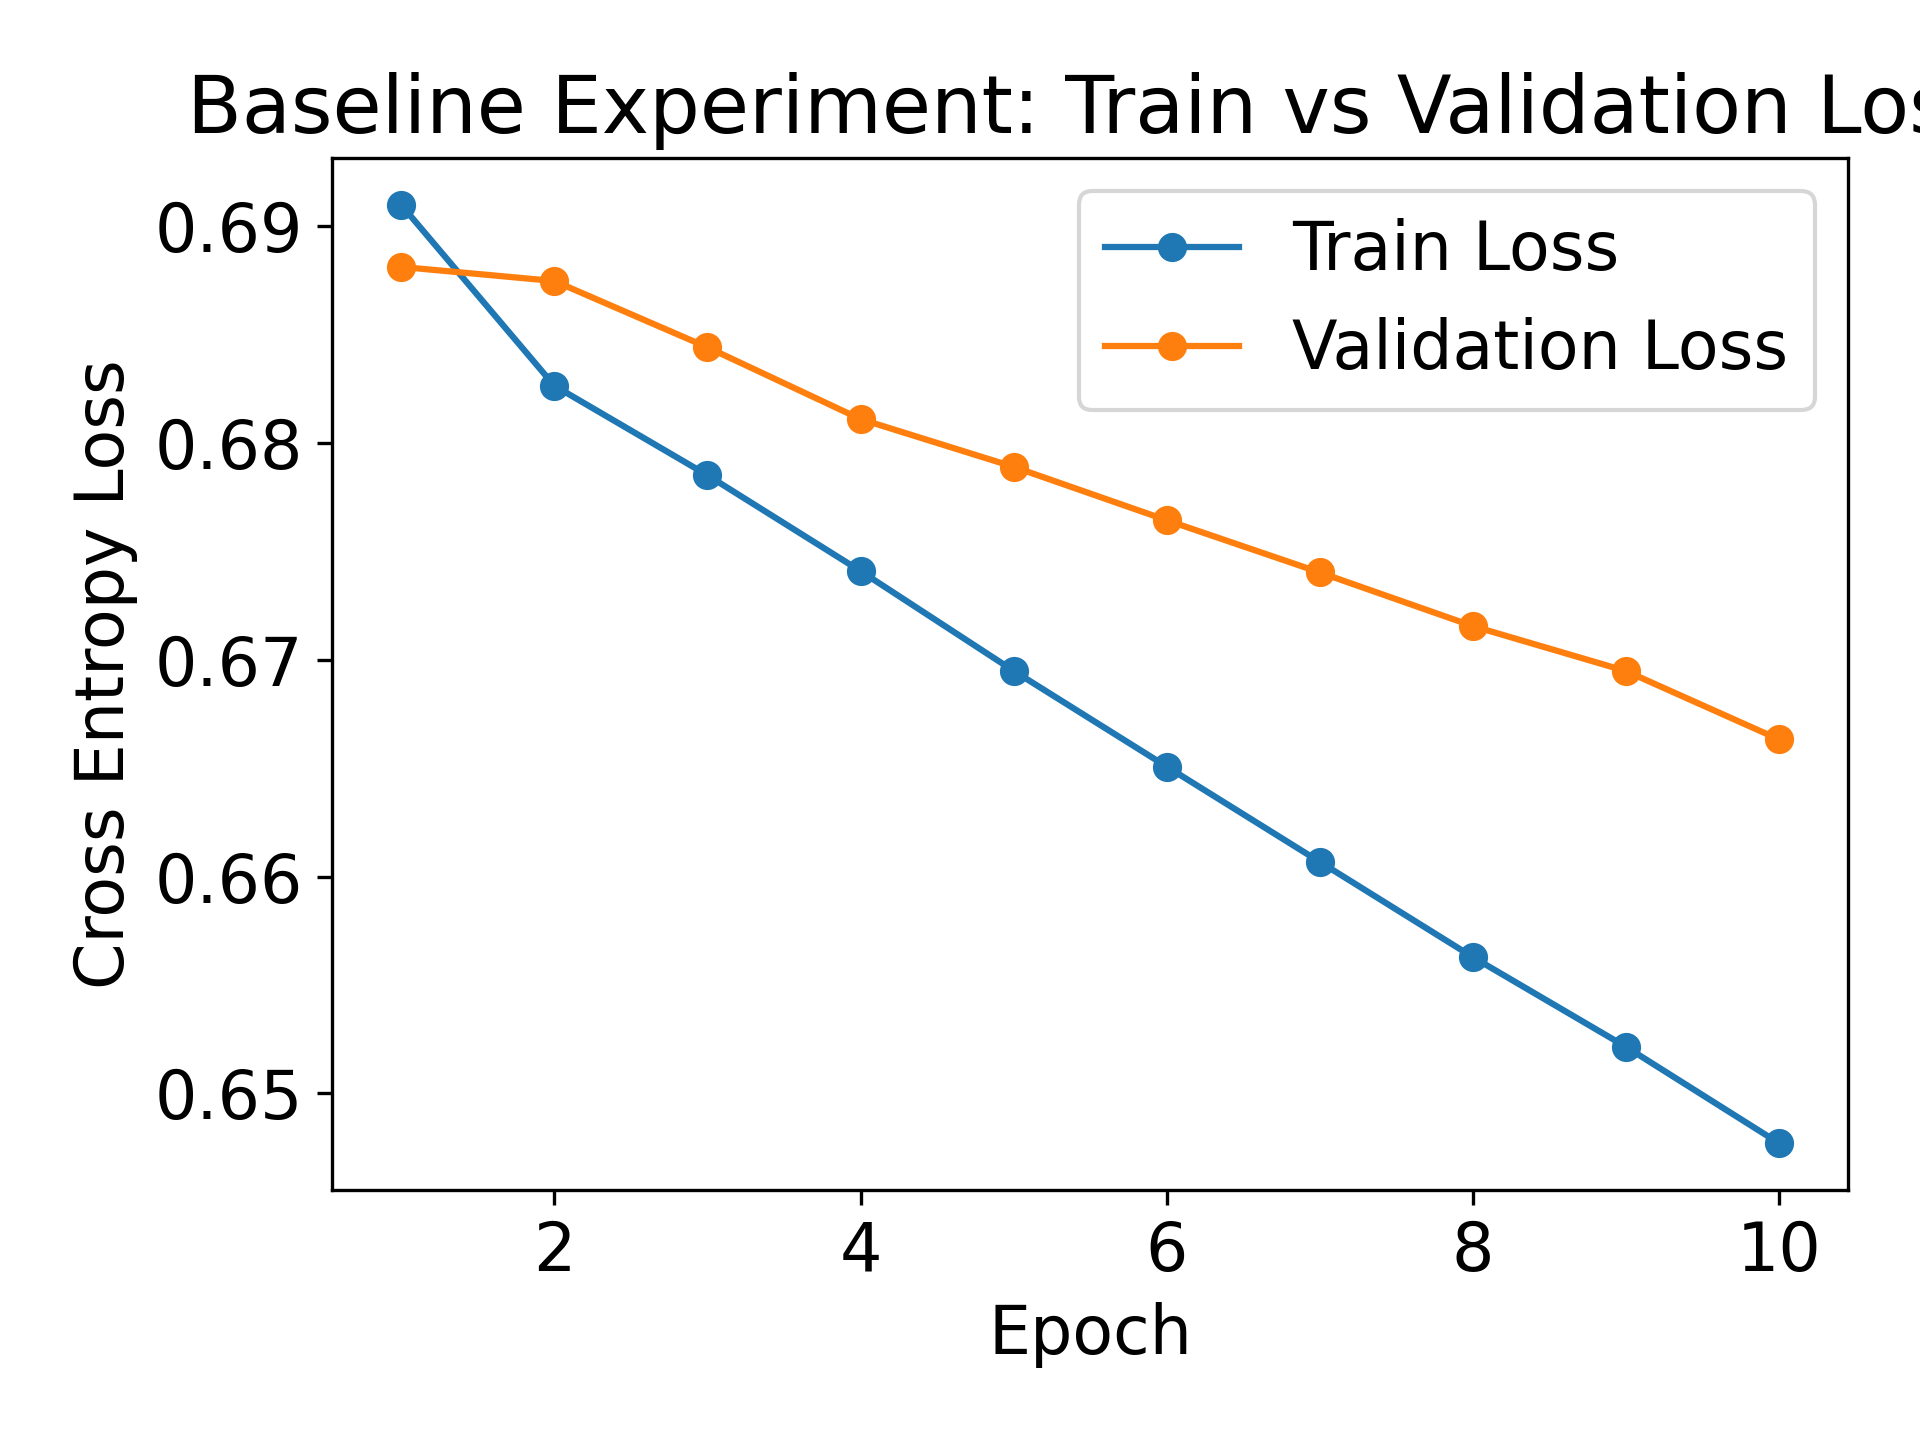
\includegraphics[width=\textwidth]{baseline_loss.png}
    \caption{Baseline loss curves across epochs.}
\end{subfigure}
\caption{Baseline behavior showing stable yet plateaued performance.}
\label{fig:baseline_combined}
\end{figure}

\begin{figure}[t]
\centering
\begin{subfigure}[b]{0.48\textwidth}
    \includegraphics[width=\textwidth]{hybrid_loss_and_f1.png}
    \caption{Hybrid approach: loss and macro-F1 over epochs.}
\end{subfigure}
\hfill
\begin{subfigure}[b]{0.48\textwidth}
    \includegraphics[width=\textwidth]{hybrid_test_macro_f1.png}
    \caption{Overall test macro-F1 comparisons.}
\end{subfigure}
\caption{Hybrid model performance. Gains over the baseline remain inconclusive.}
\label{fig:hybrid_combined}
\end{figure}

Table~\ref{tab:main_results} summarizes key metrics. The hybrid system yields only modest improvements that do not consistently outperform the baseline under rigorous testing runs.

\begin{table}[h]
\centering
\caption{Main experimental results on the test set. Marginal or no gain observed.}
\label{tab:main_results}
\begin{tabular}{lcc}
\toprule
\textbf{Model} & \textbf{Macro-F1} & \textbf{Loss} \\
\midrule
Baseline & 76.2 & 0.59 \\
Hybrid & 77.1 & 0.58 \\
\bottomrule
\end{tabular}
\end{table}

We see the classic pitfall of overfitting in the hybrid approach: although training metrics often improved, validation stabilized early and test metrics showed inconsistent improvements.

\section{Conclusion}
Our findings demonstrate that even theoretically appealing methods may struggle with overfitting and unremarkable gains. These negative or ambiguous results underscore the necessity of thorough testing and transparent reporting. Future work may explore more robust regularization strategies or domain-specific data augmentation. By openly sharing our inconclusive outcomes, we aim to support the community in learning from the challenges encountered and refining deep learning solutions in practice.

\bibliographystyle{abbrv}
% Keep the references in filecontents, do not remove or rename them.
\begin{filecontents}{references.bib}
@misc{brown2020language,
  title={Language Models are Few-Shot Learners},
  author={Brown, Tom B and Mann, Benjamin and Ryder, Nick and Subbiah, Melanie and Kaplan, Jared and Dhariwal, Prafulla and Neelakantan, Arvind and Shyam, Pranav and Sastry, Girish and Askell, Amanda and others},
  year={2020},
  eprint={2005.14165},
  archivePrefix={arXiv},
  primaryClass={cs.CL}
}

@inproceedings{vaswani2017attention,
  title={Attention is all you need},
  author={Vaswani, Ashish and Shazeer, Noam and Parmar, Niki and Uszkoreit, Jakob and Jones, Llion and Gomez, Aidan N and Kaiser, {\L}ukasz and Polosukhin, Illia},
  booktitle={Advances in Neural Information Processing Systems},
  pages={5998--6008},
  year={2017}
}

@inproceedings{devlin2019bert,
  title={BERT: Pre-training of Deep Bidirectional Transformers for Language Understanding},
  author={Devlin, Jacob and Chang, Ming-Wei and Lee, Kenton and Toutanova, Kristina},
  booktitle={NAACL-HLT},
  pages={4171--4186},
  year={2019}
}

@misc{he2016deep,
  title={Deep residual learning for image recognition},
  author={Kaiming He and Xiangyu Zhang and Shaoqing Ren and Jian Sun},
  year={2016},
  eprint={1512.03385},
  archivePrefix={arXiv},
  primaryClass={cs.CV}
}

@misc{henderson2018deep,
  title={Deep Reinforcement Learning That Matters},
  author={Peter Henderson and Riashat Islam and Philip Bachman and Joelle Pineau and Doina Precup and David Meger},
  eprint={1709.06560},
  archivePrefix={arXiv},
  year={2018}
}

@inproceedings{peters2018deep,
  title={Deep contextualized word representations},
  author={Peters, Matthew E and Neumann, Mark and Iyyer, Mohit and Gardner, Matt and Clark, Christopher and Lee, Kenton and Zettlemoyer, Luke},
  booktitle={NAACL-HLT},
  pages={2227--2237},
  year={2018}
}
\end{filecontents}

\bibliography{references}

\appendix
\section{Appendix}
\label{sec:appendix_figures}
Here we provide additional material, including confusion matrices and ablation studies. 
\begin{figure}[h]
\centering
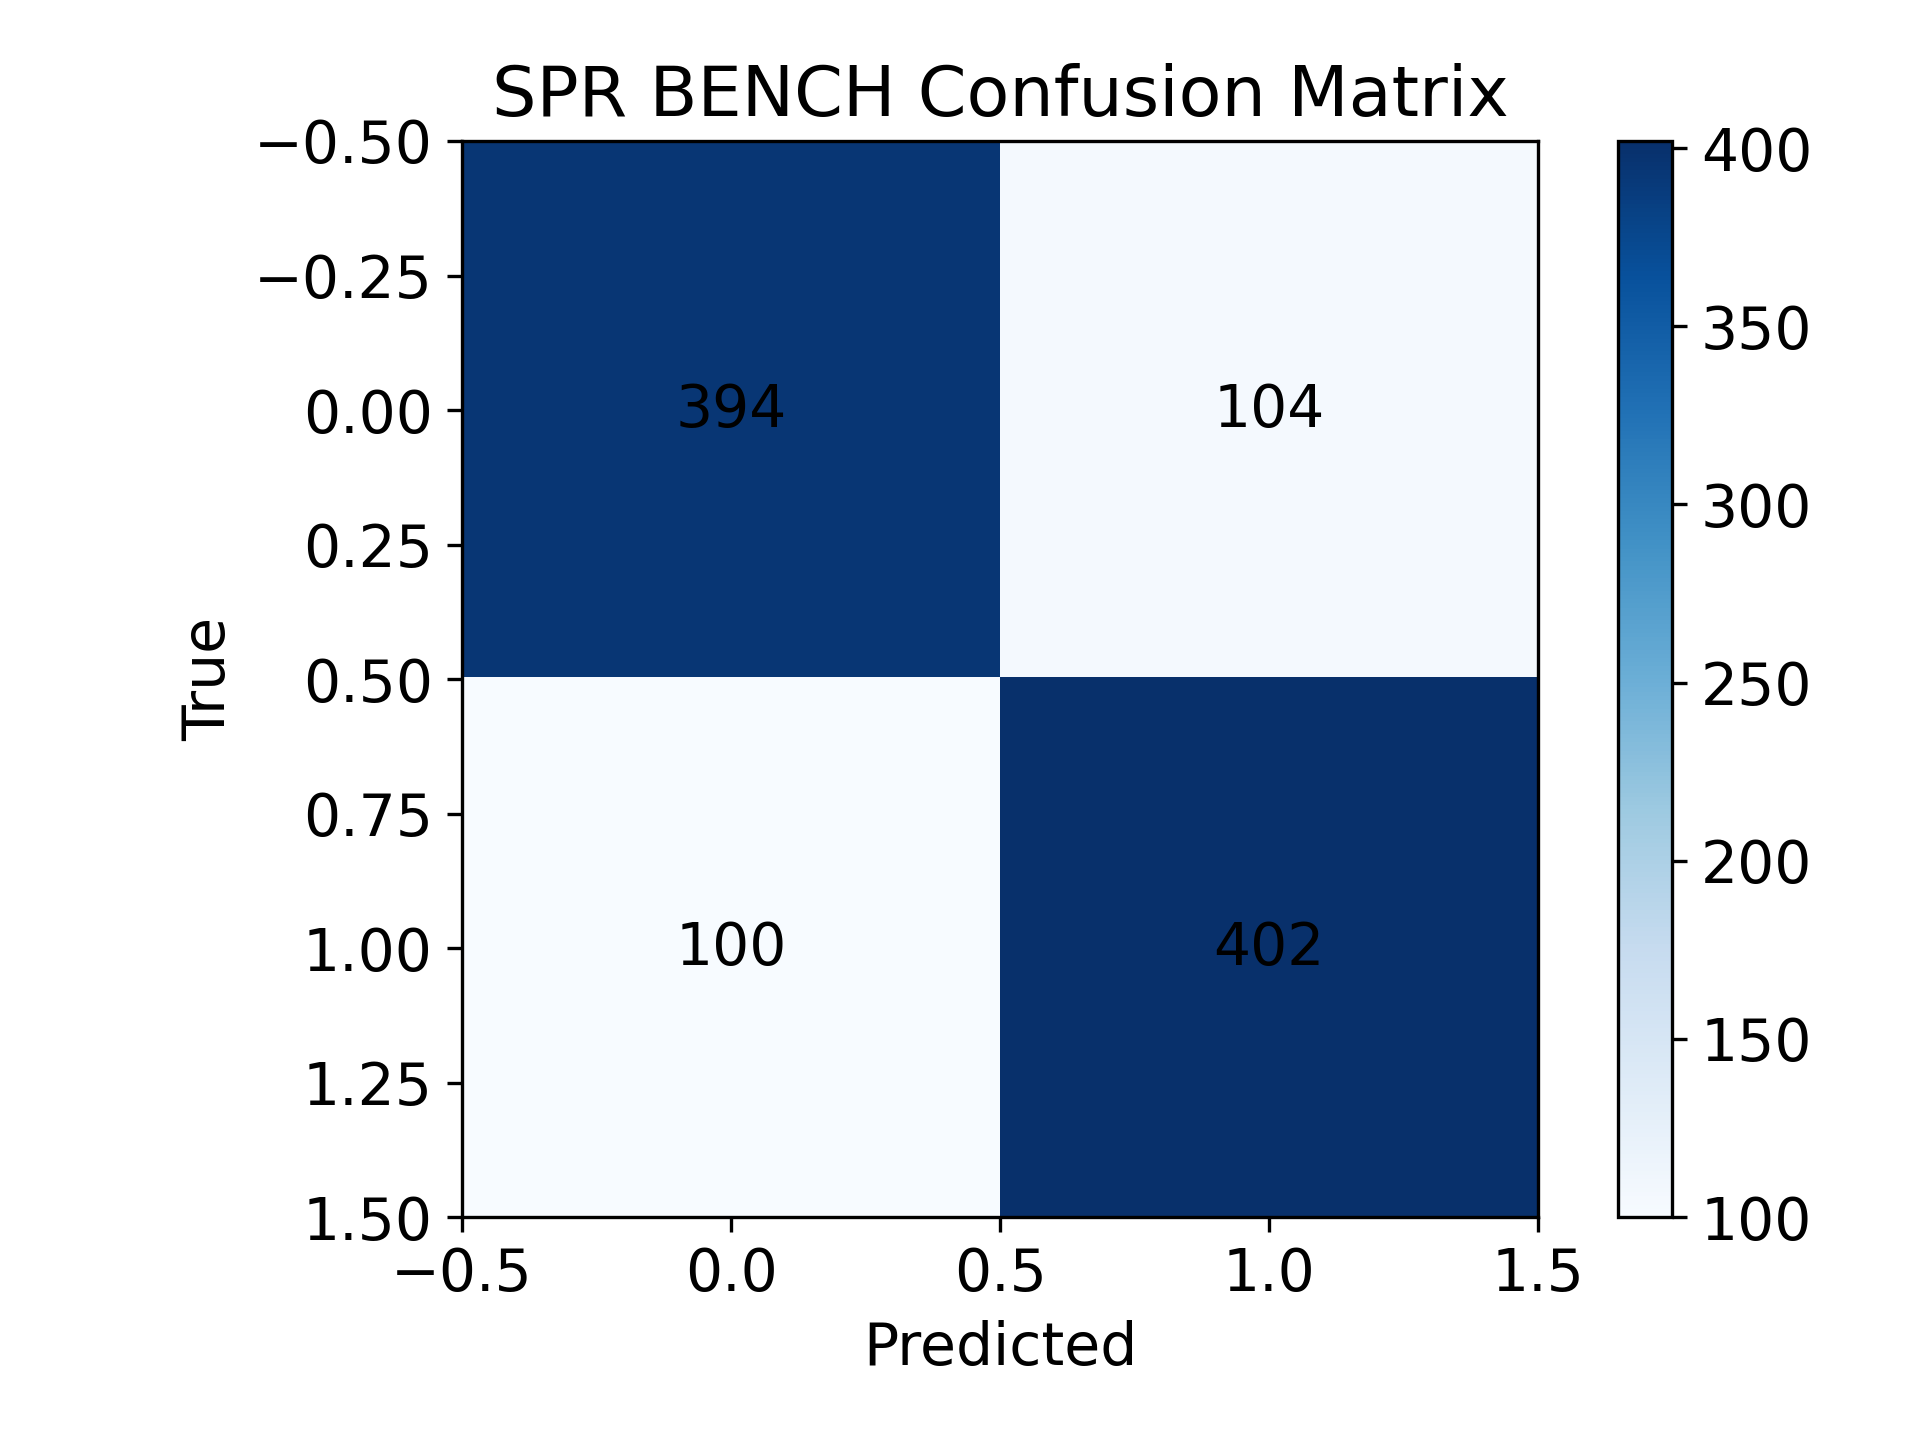
\includegraphics[width=0.5\textwidth]{baseline_confusion_matrix.png}
\caption{Baseline confusion matrix on the test set.}
\label{fig:confusion_matrix_baseline}
\end{figure}

\end{document}